\documentclass[tikz, convert={outext=.svg,pdf2svg}]{standalone}

\usepackage{tikz,amsmath,amssymb,bm,color}
\usetikzlibrary{shapes,arrows,calc,backgrounds,decorations.pathreplacing}

\definecolor{myblue}{RGB}{175, 204, 233}
\definecolor{mygreen}{RGB}{125,208,163}

\begin{document}
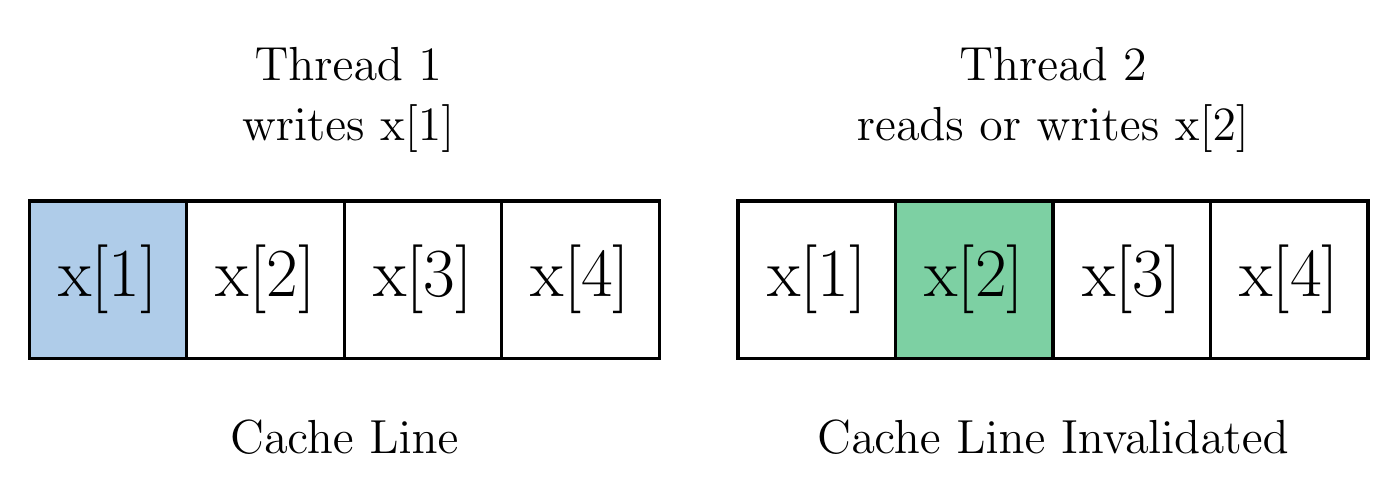
\begin{tikzpicture}

\tikzstyle{square} = [draw,outer sep=5,inner sep=3,minimum size=10,
    line width=0, very thick, draw=black!100,
    top color=white,bottom color=white]
\tikzstyle{blue} = [draw=black,outer sep=0,inner sep=0,line width=1,
    very thick, minimum width=2cm, minimum height=2cm, 
    top color=myblue, bottom color=myblue, font=\Huge, align=center]
\tikzstyle{green} = [draw=black,outer sep=0,inner sep=0,line width=1,
    very thick, minimum width=2cm, minimum height=2cm, 
    top color=mygreen, bottom color=mygreen, font=\Huge, align=center]




\node[scale=1.2] at (13.05,13.8) {\Large \begin{tabular}{c} Thread 1 \\ writes x[1] \end{tabular}};
\node[scale=1.2] at (22,13.8) {\Large \begin{tabular}{c} Thread 2 \\ reads or writes x[2] \end{tabular}};

% =========================
% four scalars - first row (flush)
% =========================
\draw[square] (9,10.5) rectangle (11,12.5);
\node[blue] at (10,11.5) {\Huge x[1]};

\draw[square] (11,10.5) rectangle (13,12.5);
\node at (12,11.5) {\Huge x[2]};


\draw[square] (13,10.5) rectangle (15,12.5);
\node at (14,11.5) {\Huge x[3]};


\draw[square] (15,10.5) rectangle (17,12.5);
\node at (16,11.5) {\Huge x[4]};


% =========================
% four scalars - second row (flush)
% =========================
\draw[square] (18,10.5) rectangle (20,12.5);
\node at (19,11.5) {\Huge x[1]};

\draw[square] (20,10.5) rectangle (22,12.5);
\node[green] at (21,11.5) {\Huge x[2]};

\draw[square] (22,10.5) rectangle (24,12.5);
\node at (23,11.5) {\Huge x[3]};

\draw[square] (24,10.5) rectangle (26,12.5);
\node at (25,11.5) {\Huge x[4]};

% plus signs between vector 1 and vector 2

\node[scale=1.2] at (13.0,9.5) {\Large Cache Line};
\node[scale=1.2] at (22.0,9.5) {\Large Cache Line Invalidated};


\end{tikzpicture}
\end{document}

